\documentclass{standalone}
\usepackage{tikz}
\usepackage{ctex,siunitx}
\usepackage{tkz-euclide}
\usepackage{amsmath}
\usetikzlibrary{patterns, calc}
\usetikzlibrary {decorations.pathmorphing, decorations.pathreplacing, decorations.shapes,}
\begin{document}
\small
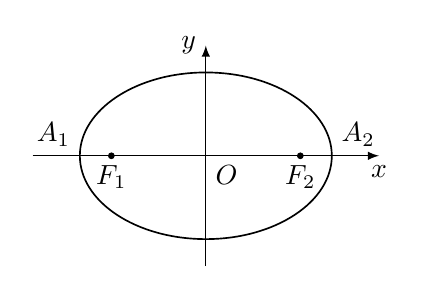
\begin{tikzpicture}[>=latex,scale=0.2]
  \draw[thin,->](-11,0)--(11,0)node[below]{$x$};
  \draw[thin,->](0,-7)--(0,7)node[left]{$y$};
  \draw[semithick](0,0)ellipse(8 and {2*sqrt(7)});
  \tkzDefPoints{0/0/O,-6/0/F1,6/0/F2}
  \tkzDrawPoints[fill=black](F1,F2)
  \tkzLabelPoint[below](F1){$F_1$}
  \tkzLabelPoint[below](F2){$F_2$}
  \tkzLabelPoints[below right](O)
  \node at (-8,0)[above left]{$A_1$};
  \node at (8,0)[above right]{$A_2$};
\end{tikzpicture}
\end{document}